\documentclass[12pt]{article}
\usepackage{graphicx} % Required for inserting images
\usepackage{makecell}
\usepackage{amsmath}
\usepackage{float}
\usepackage{algorithm}
\usepackage{verbatim}
\usepackage{moreverb}
\usepackage{hyperref}
\usepackage{booktabs}
\usepackage{geometry}
\usepackage{tabularx}
\usepackage{array}
\geometry{a4paper, margin=1in}
\usepackage[font=small,labelfont=bf]{caption} % Required for specifying captions to tables and figures
\usepackage[
backend=biber,
style=alphabetic,
]{biblatex}
\title{A bibLaTeX example}
\addbibresource{citation.bib} %Imports bibliography file
\hypersetup{
    colorlinks=true,
    linkcolor=blue,
    filecolor=magenta,      
    urlcolor=cyan,
    pdftitle={Overleaf Example},
    pdfpagemode=FullScreen,
    }

\urlstyle{same}

\title{\textbf{COVID-19 Detection Through Chest X-ray}}
\author{Lam Quoc Bao \\20127115 \and Lam Ngoc Tien \\19127574}
\date{}

\begin{document}
\maketitle
\begin{abstract}
    The SARS-CoV-2 virus gave rise to COVID-19 in late 2019 and spread quickly over the world, inflicting serious respiratory problems in a large number of individuals. Although RT-PCR assays remain the gold standard for diagnosis, their drawbacks—including false negative results and delays—led researchers to look for other approaches. The quick availability of chest X-ray and their capacity to show lung abnormalities caused by COVID-19, such as ground-glass opacities, attracted attention. This sparked the investigation into the use of machine learning approaches to improve chest X-ray COVID-19 detection, potentially providing an additional diagnostic tool in resource-constrained environments.
\end{abstract}

\maketitle

\section{Introduction}
In order to effectively limit the spread of the COVID-19 pandemic, quick and precise diagnostic techniques are required. Chest X-ray have become an essential tool of all the imaging modalities because of their accessibility and capacity to detect pulmonary involvement. This work investigates the use of cutting-edge machine learning and image processing methods to identify COVID-19 infection from chest X-ray. Our model, which we constructed using a dataset of X-ray pictures, has a high degree of accuracy in identifying COVID-19 positive and negative instances. Convolutional neural networks (CNNs) are utilized in the suggested approach to facilitate feature extraction and classification, providing a quick, easy, and inexpensive diagnostic substitute. Based on the effective triage tool this technique offers, our results show that it may help in the early diagnosis of COVID-19 and reduce the load on healthcare systems. Furthermore, the study emphasizes the significance of incorporating AI-driven solutions into the pandemic response, stressing the necessity of ongoing validation and improvement in various clinical contexts.

\subsection{Motivation}
Assessing lung involvement in COVID-19 patients may be done quickly, non-invasively, and extensively with chest X-ray. The goal of this project is to determine if machine learning approaches can be used to increase the precision and efficacy of COVID-19 detection on chest X-ray. This might lead to improved patient outcomes, early diagnosis, and optimal resource allocation. This project further aims to provide a dependable, AI-driven diagnostic tool that can be easily integrated into a variety of healthcare settings, therefore aiding in the worldwide stand to combat the pandemic.

\subsection{Practical application}
The findings of our investigation highlight he practical advantages of employing AI-driven chest X-ray analysis in COVID-19 diagnosis. We demonstrate that, in many circumstances, our approach provides faster and more accurate answers by comparing its performance with routine radiological examinations and traditional RT-PCR assays. The approach has the potential to close significant gaps in existing diagnostic methods, as evidenced by scenario-based demonstrations that mimic its application in emergency departments and rural clinics where access to RT-PCR assays may be restricted.

\subsection{Problem statement}
The rapid spread of COVID-19 has created major obstacles to prompt and precise diagnosis, especially in areas where RT-PCR testing is not readily available. Delays and technological limitations frequently hinder traditional diagnostic techniques, creating gaps in the early diagnosis and treatment of the infection. Despite being widely accessible, chest X-ray need advanced interpretation to accurately identify anomalies related to COVID-19. This study aims to provide an additional tool that can be easily integrated into current clinical workflows, particularly in resource-constrained settings. It does this by investigating the use of machine learning to improve the diagnostic accuracy of chest X-ray, addressing the urgent need for an effective, scalable solution.

\subsubsection{Input}
An input image, assign importance (learnable weights and biases) to various aspects/objects in the image and be able to differentiate one from the other.
\begin{figure}[h!]
\minipage{0.32\textwidth}
  \includegraphics[width=\linewidth]{images/patient1.png}
\endminipage\hfill
\minipage{0.32\textwidth}
  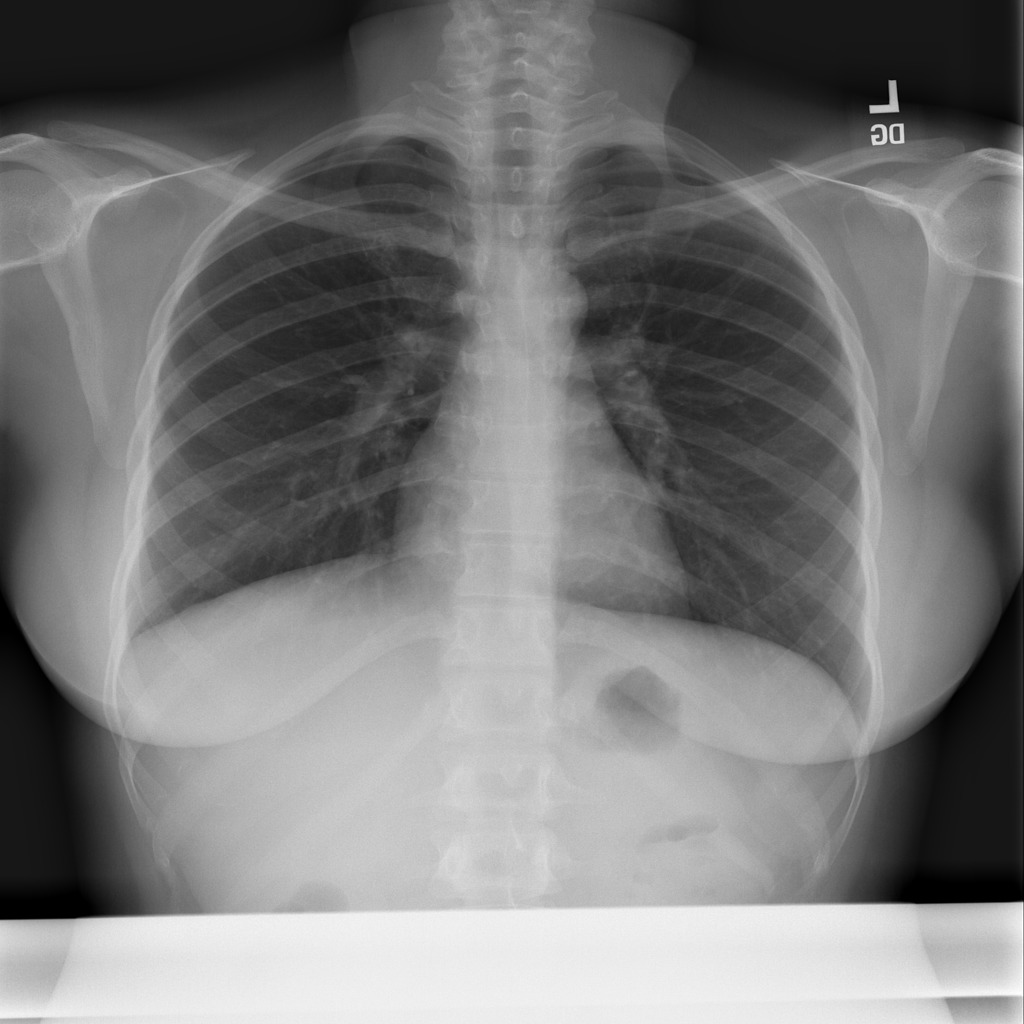
\includegraphics[width=\linewidth]{images/patient2.png}
\endminipage\hfill
\minipage{0.32\textwidth}%
  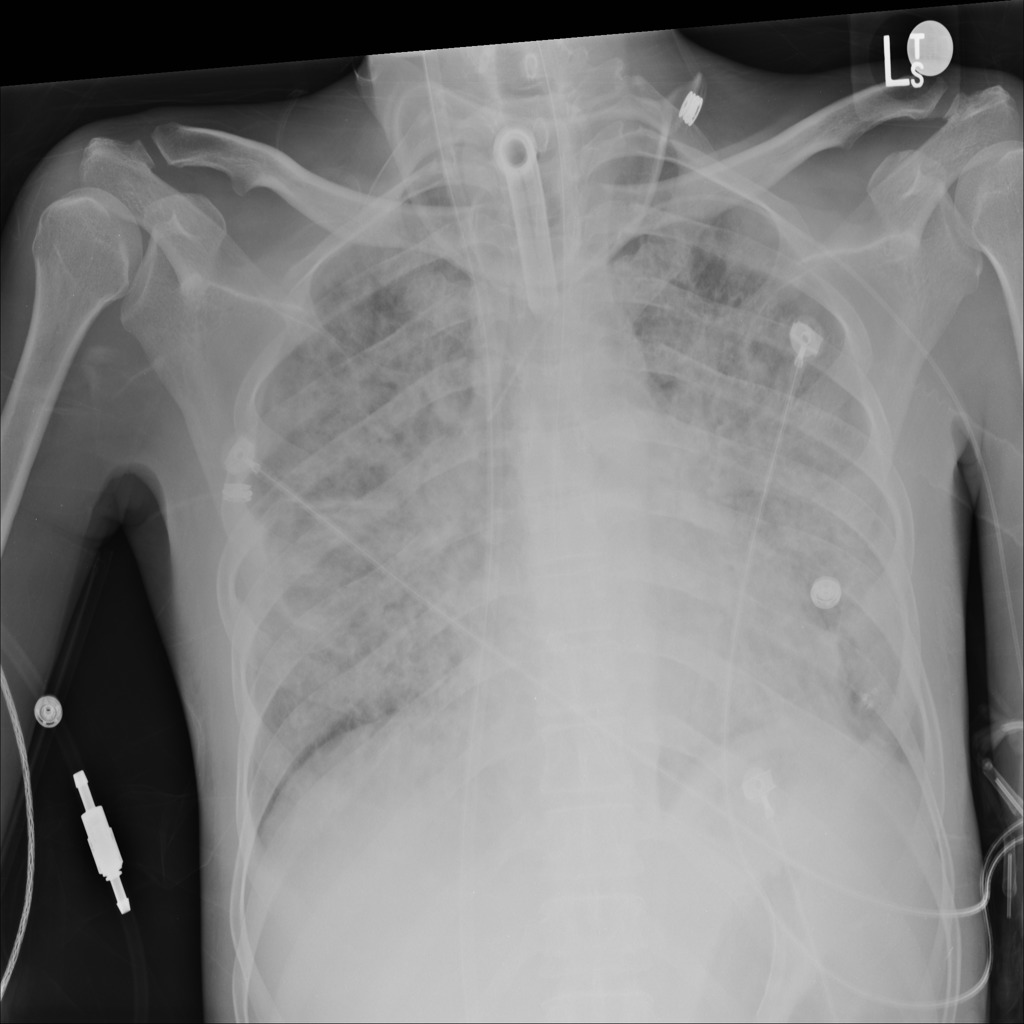
\includegraphics[width=\linewidth]{images/patient3.png}
\endminipage
\caption{Example of input images.}
\end{figure}

\subsubsection{Output}
Responding result showing the X-ray image of the patient as Normal, COVID19 or Pnemonia.
Below is an example of what we hope to achieve in this study.
\begin{center}
\begin{minipage}{\linewidth}
 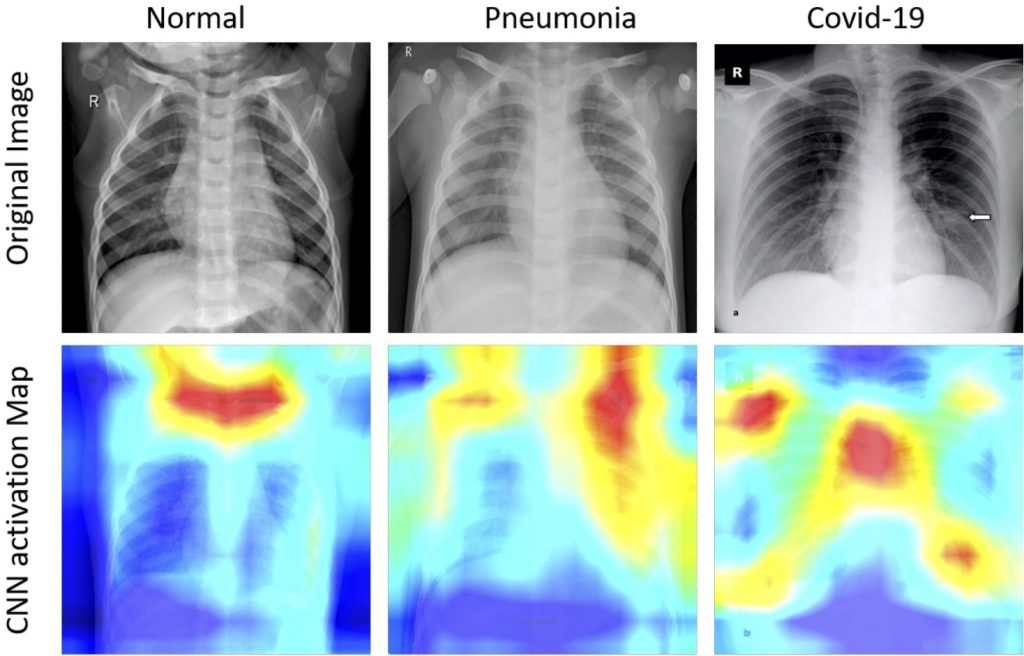
\includegraphics[width=\linewidth]{images/covid-19.jpg}
 \captionof{figure}{Example of expected output.}
\end{minipage}
\end{center}

\section{Related work}

Literature comparison of COVID-19 diagnostic methods using CXR images.
\vfill
\hfill
\begin{table}[h!]
\begin{center}
\begin{tabular}{| m {5cm} | m {4cm} | m {2cm} | m{2cm} |}
 \hline
 \textbf{Author(s)} & \textbf{Technique(s)} & \textbf{Classes Amount} & \textbf{Accuracy}\\
 \hline
 Sahinbas \& Catak [\cite{1}] & \makecell{VGG-16, VGG-19, \\ ResNet, DenseNet, \\ InceptionV3} & 2 & 80\%\\
 \hline
 Khan et al. [\cite{2}] & CoroNet & 4 & 89.6\%\\
 Ucar and Korkmaz [\cite{3}] & Bayes-SqueezeNet & 3 & 98.3\%\\
 \hline
 Jamil \& Hussain [\cite{4}] & Deep CNN & 2 & 93\%\\
 \hline
 Apostopolus et al. [\cite{5}] & VGG-19 & 3 & 93.48\%\\
 \hline
 Sethy et al. [\cite{6}] & ResNet-50 + SVM & 3 & 95.33\%\\
 \hline
 Apostolopoulos \& Mpesiana [\cite{7}] & MobileNetV2 & 3 & 96.78\%\\
 \hline
 Toraman et al. [\cite{8}] & Capsule Network & 2 & 97.24\%\\
 \hline
 Ezzat et al. [\cite{9}] & DenseNet121+GSA & 2 & 98.3\%\\
 \hline
 Saad et al. [\cite{10}] & CNN, GoogleNet, ResNet-18 & 2 & 99.3\%\\
 \hline
\end{tabular}
\end{center}
\caption{Related work table.}
\label{tab:related_work}
\end{table}
\vfill
\hfill


\section{Proposed method}
For this project, we plan to use a model based on a Convolutional Neural Network (ConvNet/CNN). CNNs are deep learning algorithms created to automatically recognize and distinguish between various features in images for processing and analysis. By training itself, a CNN can learn these filters on its own, eliminating the need for as much pre-processing as with older methods that require manual filter creation. A CNN's architecture is comparable to the way neurons are connected in the human brain, specifically the arrangement of the visual cortex. A CNN can perform an extensive analysis of an image because each neuron in the network responds to a certain region of the image called the receptive field. These regions overlap to cover the entire image.

\subsection{Model}
\begin{figure}[!htb]
    \centering
    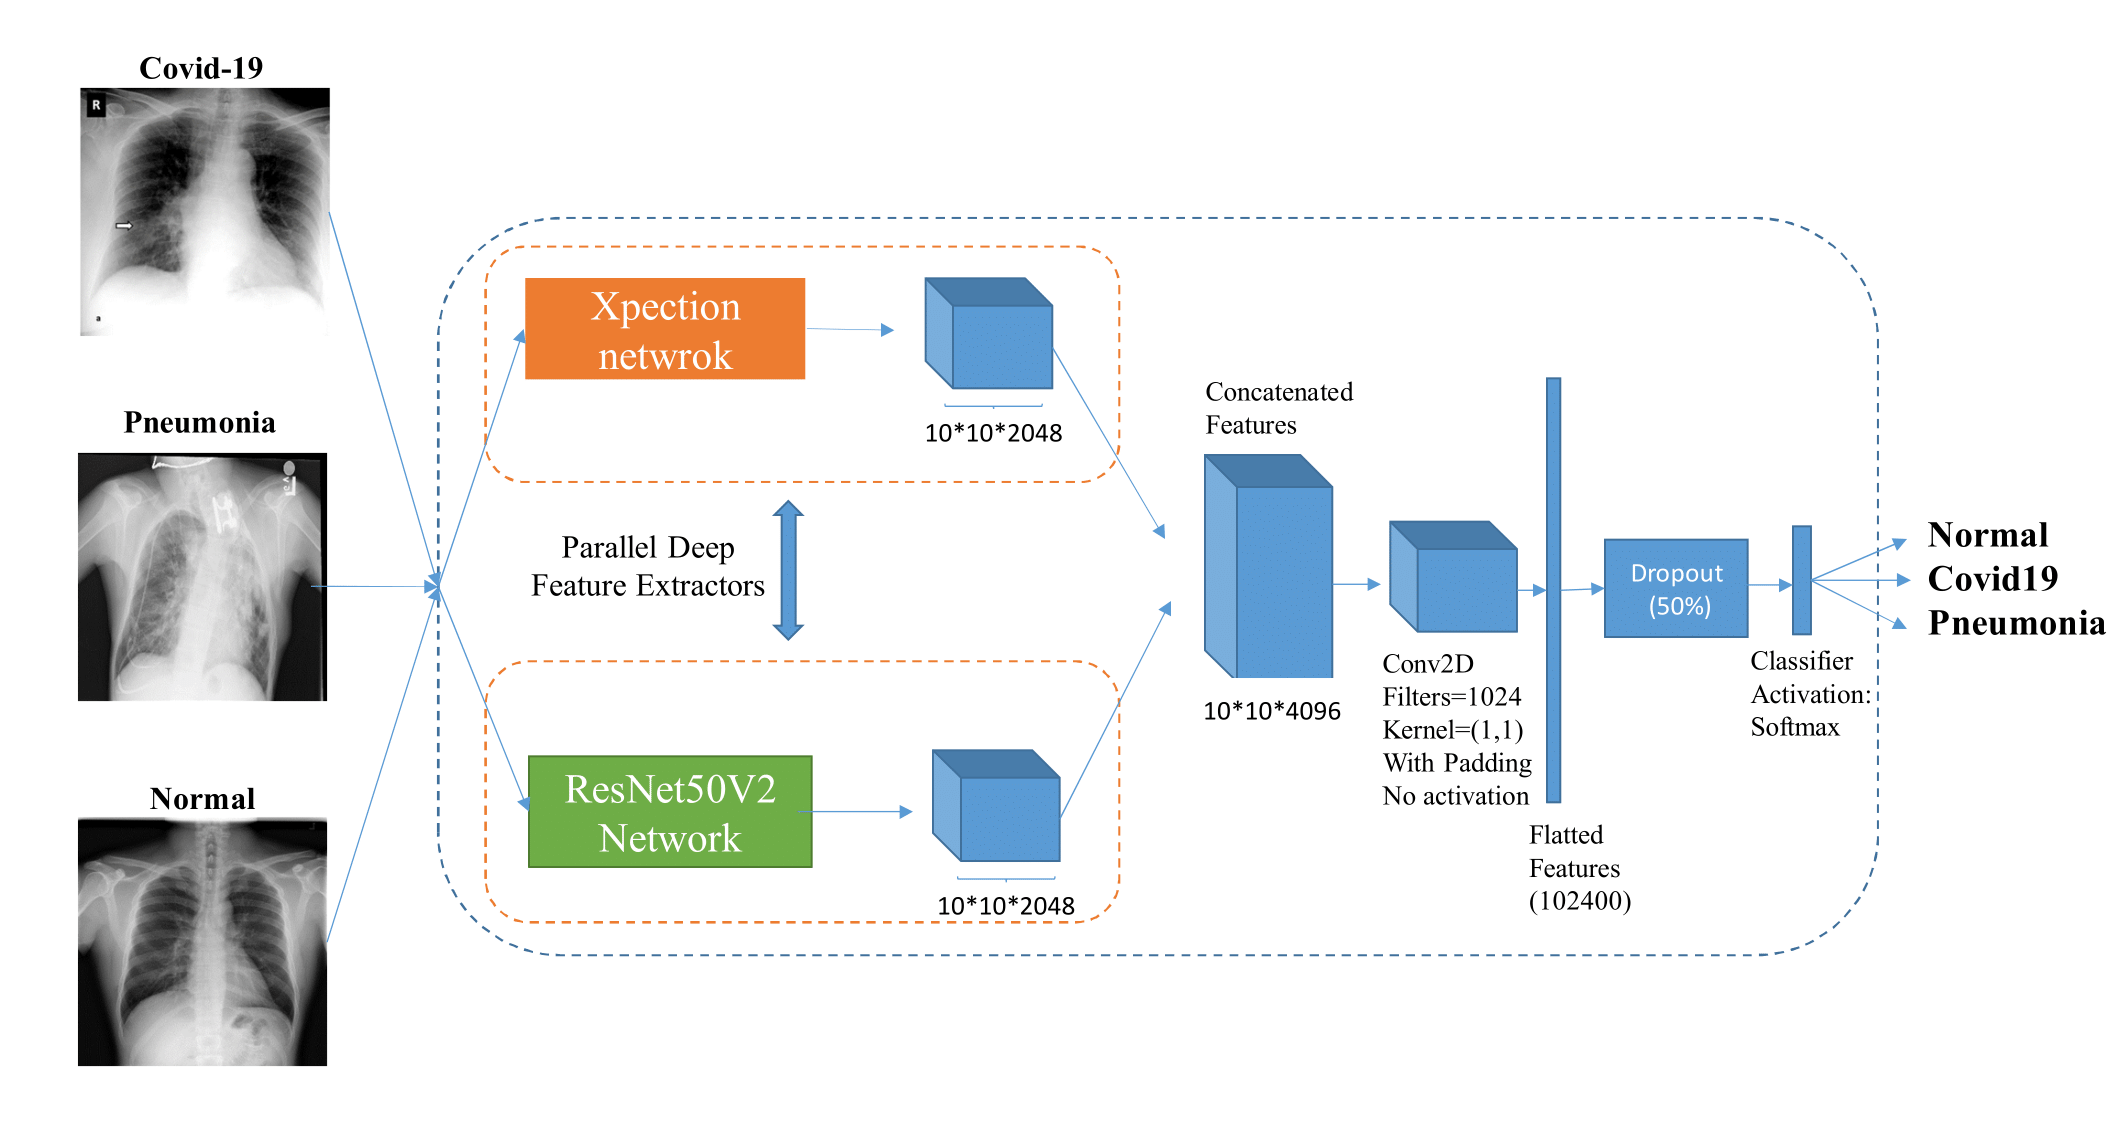
\includegraphics[width=\linewidth]{images/concatenated_net.png}
    \caption{ConvNet: CNN-based architecture of COVID-19 Detection through Chest X-ray}
    \label{fig:model}
\end{figure}
Our proposed method for COVID-19 detection using chest X-Ray begins with a series of input images, whihlinee categorized into three classes: COVID19, Pneumonia, and Normal. These images are subsequently processed through convolutional neural networks (CNNs) operating in parallel—namely, the Xception network and the ResNet50V2 network. These networks are proven effectiveness in deep feature extraction and image classification tasks.

The Xception network processes the input images by applying a series of convolutional layers, ultimately extracting deep features that are represented by a tensor of size $10 \times 10 \times 2048$. Concurrently, the same input images are passed through the ResNet50V2 network, which employs a residual learning approach to extract features. This network similarly produces a feature tensor of size $10 \times 10 \times 2048$. The parallel processing of the images through these two networks ensures that the model ultilizes the unique strengths of both architectures in extracting relevant image features.

Following feature extraction, the outputs from the Xception and ResNet50V2 networks are concatenated. This concatenation step combines the deep features from both networks into a single, larger feature set with dimensions of $10 \times 10 \times 4096$. The concatenated features are then processed through a two-dimensional convolutional layer (Conv2D) containing 1024 filters with a kernel size of $1 \times 1$. This convolutional layer is designed to further refine the combined features by emphasizing the most significant patterns within the images, while the padding ensures that the spatial dimensions are preserved. Notably, no activation function is applied at this stage to allow for the most flexible processing of the features.

Subsequent to the Conv2D layer, the features are flattened into a one-dimensional vector with a size of 102,400. This flattened vector represents the essential characteristics of the input image in a format suitable for classification. To mitigate the risk of overfitting and enhance the model's generalization capability, a dropout layer with a rate of 50\% is applied. This layer randomly disables half of the neurons during the training phase, which helps in preventing the model from becoming too dependent on any particular features.

The final classification step is carried out by a fully connected layer that utilizes the Softmax activation function. This classifier processes the flattened features and produces a probability distribution across the three target classes: Normal, COVID-19, and Pneumonia. The output of the Softmax layer determines the predicted class for each input chest X-ray and provide a reliable diagnostic tool for identifying COVID-19, telling it apart from other types of pneumonia and normal cases.

\subsection{Loss function}
This study optimizes the COVID-19 detection model based on chest X-ray using the categorical cross-entropy loss function. When assigning each input to one of multiple discrete categories—in this case, Normal, COVID-19, or Pneumonia—in multi-class classification problems, categorical cross-entropy is especially well-suited. The model is trained to minimize the difference between the true distribution and the predicted distribution, as determined by the loss function. In particular, categorical cross-entropy penalizes the model more severely when the projected probability for the correct class is low. It does this by comparing the predicted probabilities (the output of the Softmax layer) for each class with the actual class labels.
Mathematically, the categorical cross-entropy loss function is defined as:

\begin{equation}
L= -\sum_{i=1}^N\sum_{c=1}^Cy_{i,c}\log(\hat{y}_{i,c})
\end{equation}

where N represents the number of samples in the batch, C denotes the number of classes (in this case, 3: Normal, COVID-19, and Pneumonia), \begin{math}y_{i,c}\end{math} is the binary indicator (0 or 1) if class label c is the correct classification for sample i and \begin{math}\hat{y}_{i,c}\end{math} is the predicted probability that sample i belongs to class c. The loss function sums the negative logarithm of the predicted probability for the true class over all classes and samples, which pushed the model to produce higher probabilities for the correct classes and lower probabilities for the incorrect ones.

\section{Experiments}
In this section, we present the experimental setup used to evaluate the performance of our proposed COVID-19 detection model based on chest X-ray. We describe the datasets utilized, the preprocessing steps undertaken, the model architecture configurations, and the training protocols employed. Additionally, we detail the evaluation metrics and the experimental conditions under which the model was tested. These experiments are designed to assess how well the model can classify chest X-ray images into three categories: Normal, COVID-19, and Pneumonia.

\subsection{Dataset}
The model was trained using data from the following Github link. Specifically, the dataset used in this COVID-Net research from the Github page is referred to as the "COVIDx Dataset," which was curated and released by Linda Wang and Alexander Wong. This dataset is a combination of several publicly available chest X-ray datasets, merged and annotated for the purpose of COVID-19 detection using deep learning models.

\subsection{Metric}
We reported the four different metrics for evaluating our network for each of the three class as follows:\\
Accuracy (each class) = \begin{math}\frac{\text{TP + TN}}{\text{TP + FP + TN + FN}}\end{math}\\
Specificity = \begin{math}\frac{\text{TN}}{\text{FP + TN}}\end{math}\\
Sensitivity = \begin{math}\frac{\text{TP}}{\text{TP + FN}}\end{math}\\
Precision = \begin{math}\frac{\text{TP}}{\text{TP + FP}}\end{math}\\

\subsection{Experimental setup}
With our chosen dataset and metric, we proceeded with the following training preparation. This diagram outlines a comprehensive framework for training and validating a neural network for the detection of COVID-19 and pneumonia using chest X-ray images. Below is a step-by-step explanation of the framework:

\newpage
\vfill
\begin{figure}[!hb]
    \centering
    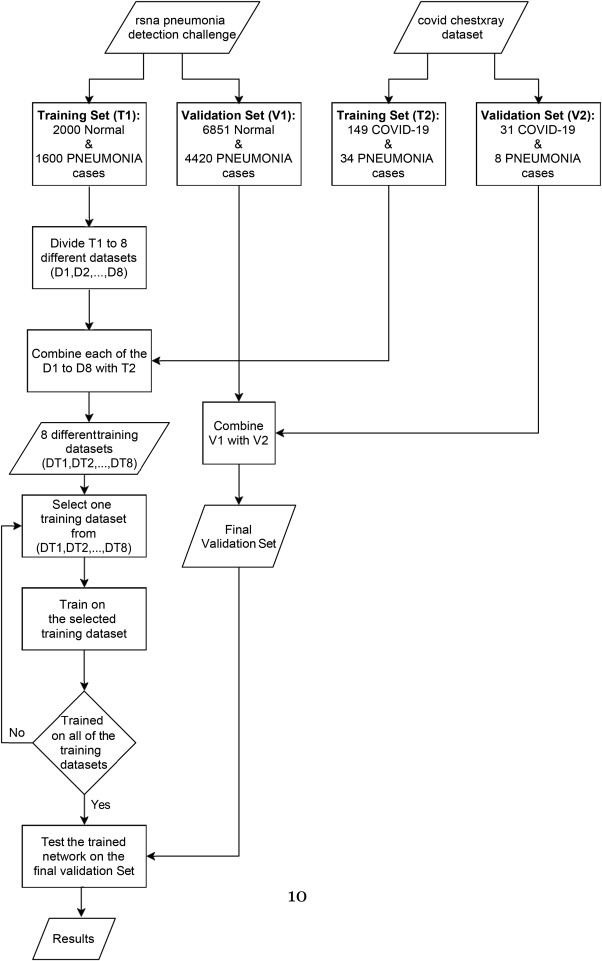
\includegraphics[width=\linewidth]{images/framework.jpg}
    \caption{Our training model framework.}
    \label{fig:training}
\end{figure}
\vfill
\clearpage

\textbf{Dataset Preparation:} The framework utilizes two primary datasets: the RSNA Pneumonia Detection Challenge dataset and the COVID-19 Chest X-ray dataset. The RSNA dataset is divided into a training set (T1) containing 2,000 normal cases and 1,600 pneumonia cases, and a validation set (V1) with 6,851 normal cases and 4,420 pneumonia cases. The COVID-19 dataset is also divided into a training set (T2) containing 149 COVID-19 cases and 34 pneumonia cases, and a validation set (V2) with 31 COVID-19 cases and 8 pneumonia cases.

\textbf{Training Set Augmentation:} The training set T1 from the RSNA dataset is further divided into eight different subsets, labeled D1 through D8. Each of these subsets is then combined with the training set T2 from the COVID-19 dataset. This process results in eight distinct training datasets, labeled DT1 through DT8.

\textbf{Training Process:} One of the combined training datasets (DT1 to DT8) is selected for training the neural network. The model is trained on the selected dataset. This process is iterated, ensuring that the network is trained on each of the eight training datasets sequentially.

\textbf{Validation Process:} The validation sets V1 from the RSNA dataset and V2 from the COVID-19 dataset are combined to form a final validation set. After the model has been trained on all eight training datasets, it is tested on this final validation set to evaluate its performance.

\textbf{Evaluation and Results:} The trained network's performance is assessed on the final validation set, and the results are recorded. This step is crucial for determining the effectiveness of the training process and the generalizability of the model to unseen data.

This process ensures that the model is trained and validated using a comprehensive approach, incorporating diverse datasets and rigorous validation to improve its accuracy in detecting COVID-19 and pneumonia from chest X-ray images.

\subsection{Experimental results}
Results from our model are then recorded within these tables.

\vfill
\hfill
% Table 1: Sensitivity Results
\begin{table}[h!]
\centering
\renewcommand{\arraystretch}{1.0}  % Increased row height for better readability
\setlength{\tabcolsep}{4pt}  % Further increased spacing between columns
\resizebox{\textwidth}{!}{  % Resizing the table to take the full width of the page
\begin{tabularx}{\textwidth}{c *{4}{>{\centering\arraybackslash}X}}
\toprule
\textbf{Fold} & \textbf{Network} & \textbf{COVID-19 Sensitivity} & \textbf{PNEUMONIA Sensitivity} & \textbf{NORMAL Sensitivity} \\
\midrule
1 & Xception & 83.87 & 90.11 & 91.15 \\
  & ResNet50V2 & 87.09 & 87.28 & 92.45 \\
  & Concatenated & 83.87 & 84.72 & 95.25 \\
2 & Xception & 74.19 & 87.64 & 93.79 \\
  & ResNet50V2 & 70.96 & 82.78 & 92.54 \\
  & Concatenated & 74.19 & 88.52 & 93.60 \\
3 & Xception & 70.00 & 89.18 & 93.57 \\
  & ResNet50V2 & 73.33 & 85.29 & 93.89 \\
  & Concatenated & 83.33 & 87.03 & 94.90 \\
4 & Xception & 70.96 & 86.38 & 93.57 \\
  & ResNet50V2 & 70.96 & 90.83 & 88.52 \\
  & Concatenated & 83.87 & 87.33 & 92.54 \\
5 & Xception & 67.74 & 91.42 & 92.46 \\
  & ResNet50V2 & 67.74 & 81.53 & 95.59 \\
  & Concatenated & 77.41 & 89.16 & 94.03 \\
Average & Xception & 73.35 & 88.95 & 92.91 \\
 & ResNet50V2 & 74.02 & 85.54 & 92.60 \\
 & Concatenated & 80.53 & 87.35 & 94.06 \\
\bottomrule
\end{tabularx}}
\caption{Sensitivity Results of various networks across different folds for COVID-19, PNEUMONIA, and NORMAL.}
\end{table}

% Table 2: Specificity Results
\begin{table}[h!]
\centering
\renewcommand{\arraystretch}{1.0}  % Increased row height for better readability
\setlength{\tabcolsep}{4pt}  % Further increased spacing between columns
\resizebox{\textwidth}{!}{  % Resizing the table to take the full width of the page
\begin{tabularx}{\textwidth}{c *{4}{>{\centering\arraybackslash}X}}
\toprule
\textbf{Fold} & \textbf{Network} & \textbf{COVID-19 Specificity} & \textbf{PNEUMONIA Specificity} & \textbf{NORMAL Specificity} \\
\midrule
1 & Xception & 99.1 & 91.73 & 91.51 \\
  & ResNet50V2 & 99.15 & 93.03 & 88.61 \\
  & Concatenated & 99.4 & 95.51 & 85.89 \\
2 & Xception & 99.63 & 94.06 & 88.14 \\
  & ResNet50V2 & 99.41 & 92.72 & 83.98 \\
  & Concatenated & 99.76 & 93.69 & 88.95 \\
3 & Xception & 99.75 & 93.66 & 89.60 \\
  & ResNet50V2 & 99.14 & 94.30 & 86.81 \\
  & Concatenated & 99.69 & 95.03 & 87.64 \\
4 & Xception & 99.63 & 93.71 & 87.06 \\
  & ResNet50V2 & 99.31 & 88.99 & 81.82 \\
  & Concatenated & 99.32 & 93.03 & 88.34 \\
5 & Xception & 99.64 & 92.71 & 91.87 \\
  & ResNet50V2 & 99.63 & 95.87 & 81.98 \\
  & Concatenated & 99.62 & 94.33 & 89.62 \\
Average & Xception & 99.55 & 91.73 & 89.63 \\
 & ResNet50V2 & 99.33 & 92.93 & 86.64 \\
 & Concatenated & 99.56 & 94.32 & 89.80 \\
\bottomrule
\end{tabularx}}
\caption{Specificity Results of various networks across different folds for COVID-19, PNEUMONIA, and NORMAL.}
\end{table}
\clearpage
\newpage
% Table 3: Accuracy Results
\begin{table}[h!]
\centering
\renewcommand{\arraystretch}{0.9}  % Increased row height for better readability
\setlength{\tabcolsep}{4pt}  % Further increased spacing between columns
\resizebox{\textwidth}{!}{  % Resizing the table to take the full width of the page
\begin{tabularx}{\textwidth}{c *{4}{>{\centering\arraybackslash}X}}
\toprule
\textbf{Fold} & \textbf{Network} & \textbf{COVID-19 Accuracy} & \textbf{PNEUMONIA Accuracy} & \textbf{NORMAL Accuracy} \\
\midrule
1 & Xception & 99.06 & 91.10 & 91.29 \\
  & ResNet50V2 & 99.12 & 90.78 & 90.94 \\
  & Concatenated & 99.35 & 91.29 & 91.57 \\
2 & Xception & 99.56 & 91.55 & 91.57 \\
  & ResNet50V2 & 99.33 & 88.83 & 89.17 \\
  & Concatenated & 99.69 & 91.67 & 91.77 \\
3 & Xception & 99.67 & 91.91 & 92.01 \\
  & ResNet50V2 & 99.07 & 90.78 & 91.11 \\
  & Concatenated & 99.65 & 91.90 & 92.04 \\
4 & Xception & 99.55 & 90.84 & 91.01 \\
  & ResNet50V2 & 99.23 & 89.71 & 89.82 \\
  & Concatenated & 99.27 & 90.80 & 90.89 \\
5 & Xception & 99.55 & 92.20 & 92.23 \\
  & ResNet50V2 & 99.54 & 90.27 & 90.23 \\
  & Concatenated & 99.56 & 92.31 & 92.29 \\
Average & Xception & 99.48 & 91.52 & 91.62 \\
 & ResNet50V2 & 99.26 & 90.97 & 90.25 \\
 & Concatenated & 99.50 & 91.60 & 91.71 \\
\bottomrule
\end{tabularx}}
\caption{Accuracy Results of various networks across different folds for COVID-19, PNEUMONIA, and NORMAL.}
\end{table}

% Table 4: Precision Results
\begin{table}[h!]
\centering
\renewcommand{\arraystretch}{1.0}  % Increased row height for better readability
\setlength{\tabcolsep}{4pt}  % Further increased spacing between columns
\resizebox{\textwidth}{!}{  % Resizing the table to take the full width of the page
\begin{tabularx}{\textwidth}{c *{4}{>{\centering\arraybackslash}X}}
\toprule
\textbf{Fold} & \textbf{Network} & \textbf{COVID-19 Precision} & \textbf{PNEUMONIA Precision} & \textbf{NORMAL Precision} \\
\midrule
1 & Xception & 20.47 & 87.50 & 94.29 \\
  & ResNet50V2 & 21.95 & 88.93 & 92.58 \\
  & Concatenated & 27.65 & 92.37 & 91.22 \\
2 & Xception & 35.38 & 90.45 & 92.40 \\
  & ResNet50V2 & 24.71 & 87.95 & 89.89 \\
  & Concatenated & 46.00 & 90.01 & 92.87 \\
3 & Xception & 42.85 & 90.04 & 93.26 \\
  & ResNet50V2 & 18.48 & 90.58 & 91.63 \\
  & Concatenated & 41.66 & 91.83 & 92.20 \\
4 & Xception & 34.37 & 89.81 & 91.75 \\
  & ResNet50V2 & 22.00 & 84.11 & 94.33 \\
  & Concatenated & 25.24 & 88.94 & 92.43 \\
5 & Xception & 33.87 & 88.95 & 94.59 \\
  & ResNet50V2 & 33.33 & 92.69 & 89.08 \\
  & Concatenated & 35.82 & 90.99 & 93.22 \\
Average & Xception & 33.39 & 89.35 & 95.02 \\
 & ResNet50V2 & 24.09 & 88.85 & 91.50 \\
 & Concatenated & 35.27 & 90.89 & 93.63 \\
\bottomrule
\end{tabularx}}
\caption{Precision Results of various networks across different folds for COVID-19, PNEUMONIA, and NORMAL.}
\end{table}
\vfill
\hfill

\subsection{How to run your code}
These library versions are required to run our source code.\\
\begin{boxedverbatim}
flask==3.0.3
tensorflow==2.9.0
opencv-python==4.10.0.84
keras==2.9.0
numpy==1.26.4 
\end{boxedverbatim}
\bigskip
\\

Below are steps needed to run our source code. A demonstration video for visualized guide at the end of this section.
\bigskip
\\

1. Clone the repository:\\
\begin{boxedverbatim}
   ```bash
   git clone https://github.com/lltlien/covid19-xray-detection-flask-app.git
   cd covid19-xray-detection-flask-app
\end{boxedverbatim}
\bigskip
\\
2. Create and activate a virtual environment:\\
\begin{boxedverbatim}
    ```bash
    virtualenv venv
    source venv/bin/activate  # On Windows, use `venv\Scripts\activate`
\end{boxedverbatim}
\bigskip
\\
3. Install the required packages:\\
\begin{boxedverbatim}
    ```bash
    pip install -r requirements.txt
\end{boxedverbatim}
\bigskip
\\
4. Download model to `covid19-xray-detection-flask-app` folder in \href{https://github.com/lltlien/covid19-xray-detection-flask-app/releases/download/lastest/concatenate-fold3.hdf5}{this link}. 
\bigskip
\\

5. Run the application:\\
\begin{boxedverbatim}
    ```bash
    python3 app.py
\end{boxedverbatim}
\bigskip
\\
6. Open your web browser and go to http://127.0.0.1:5000/ to use the app.\\
\begin{boxedverbatim}
<p align="center">
	<img src="static/web1.png" alt="photo not available" width="100%" height="70%">
	<br>
	<img src="static/web2.png" alt="photo not available" width="100%" height="70%">
	<br>
    <em>The simple web app</em>

</p>
\end{boxedverbatim}
\bigskip
\\

7. Successfully setup should allow you to have this website page opened.
\begin{center}
\begin{minipage}{\linewidth}
    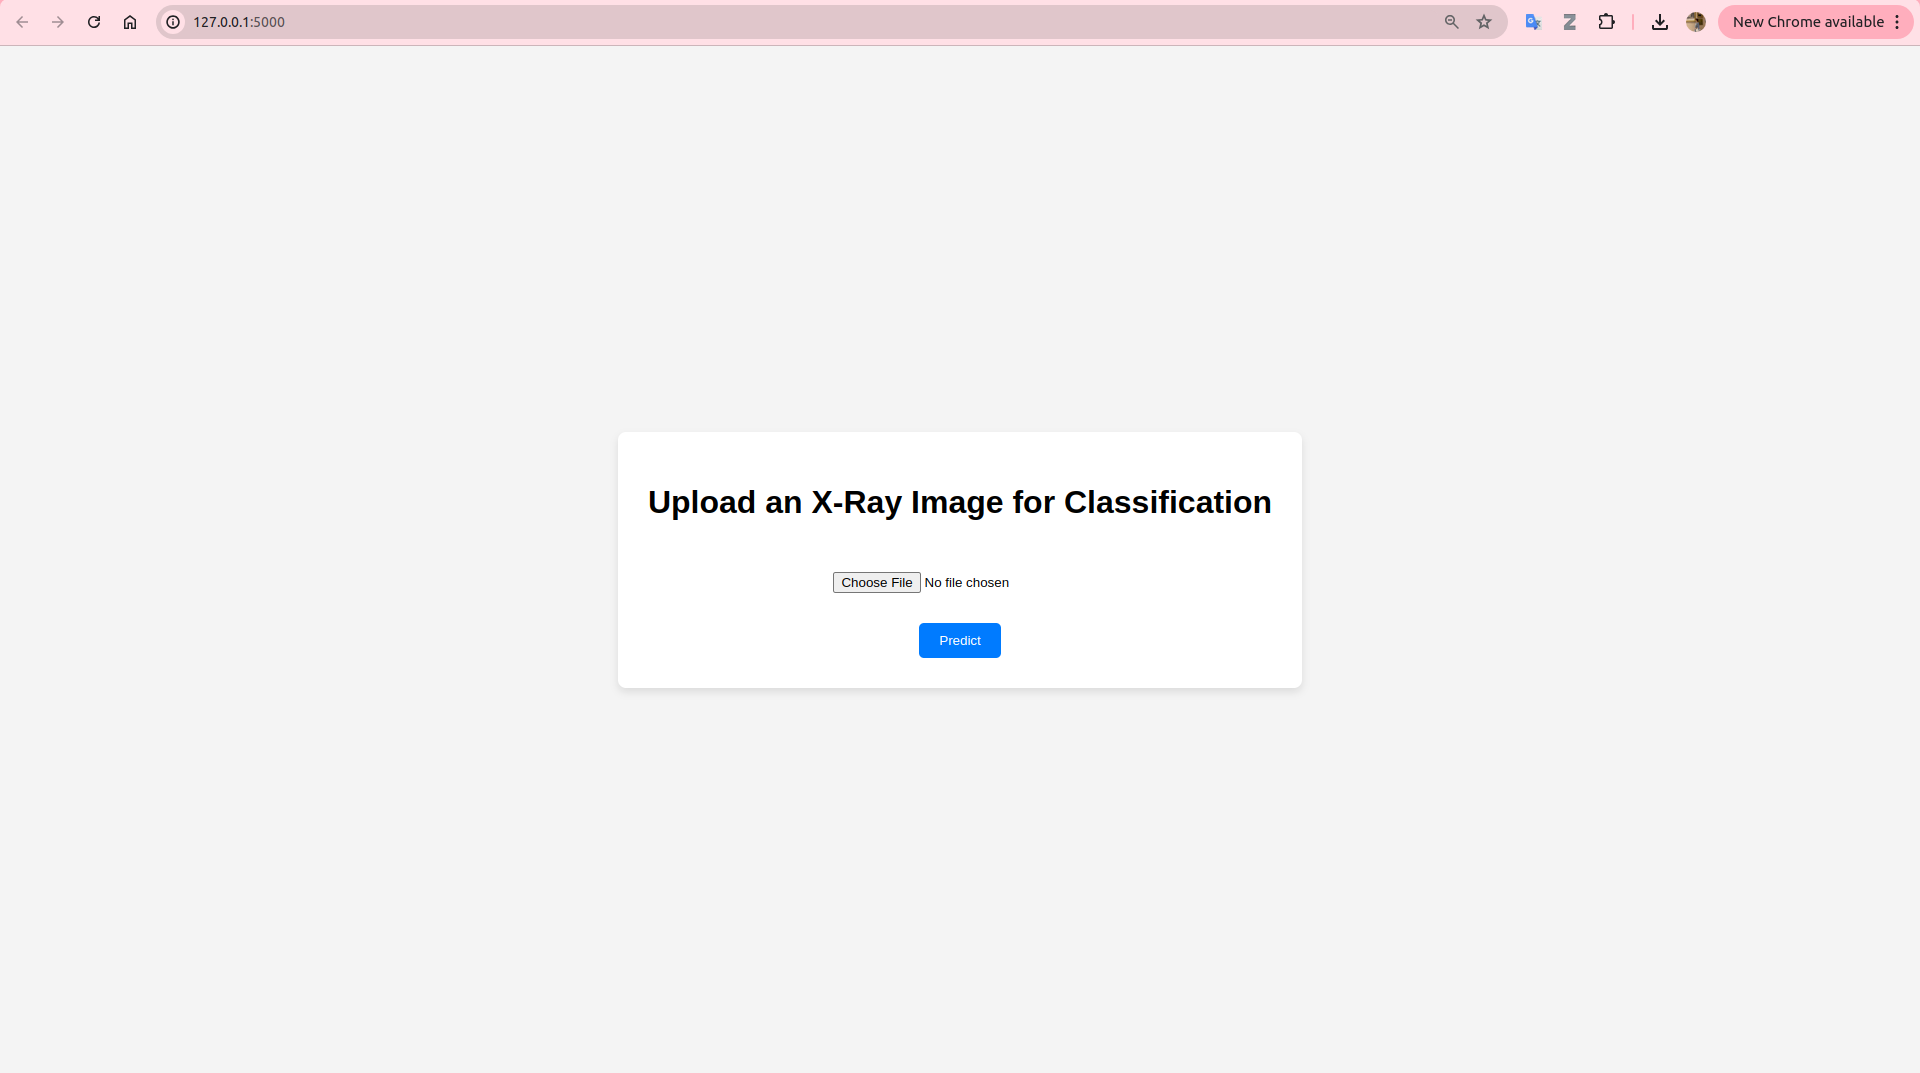
\includegraphics[width=\linewidth]{images/web1.png}
    \captionof{figure}{Homepage of our source code.}
    \label{fig:input-code}
\end{minipage}
\end{center}

8. Add an image X-ray of your choice and get the result.\\
\begin{center}
\begin{minipage}{\linewidth}
    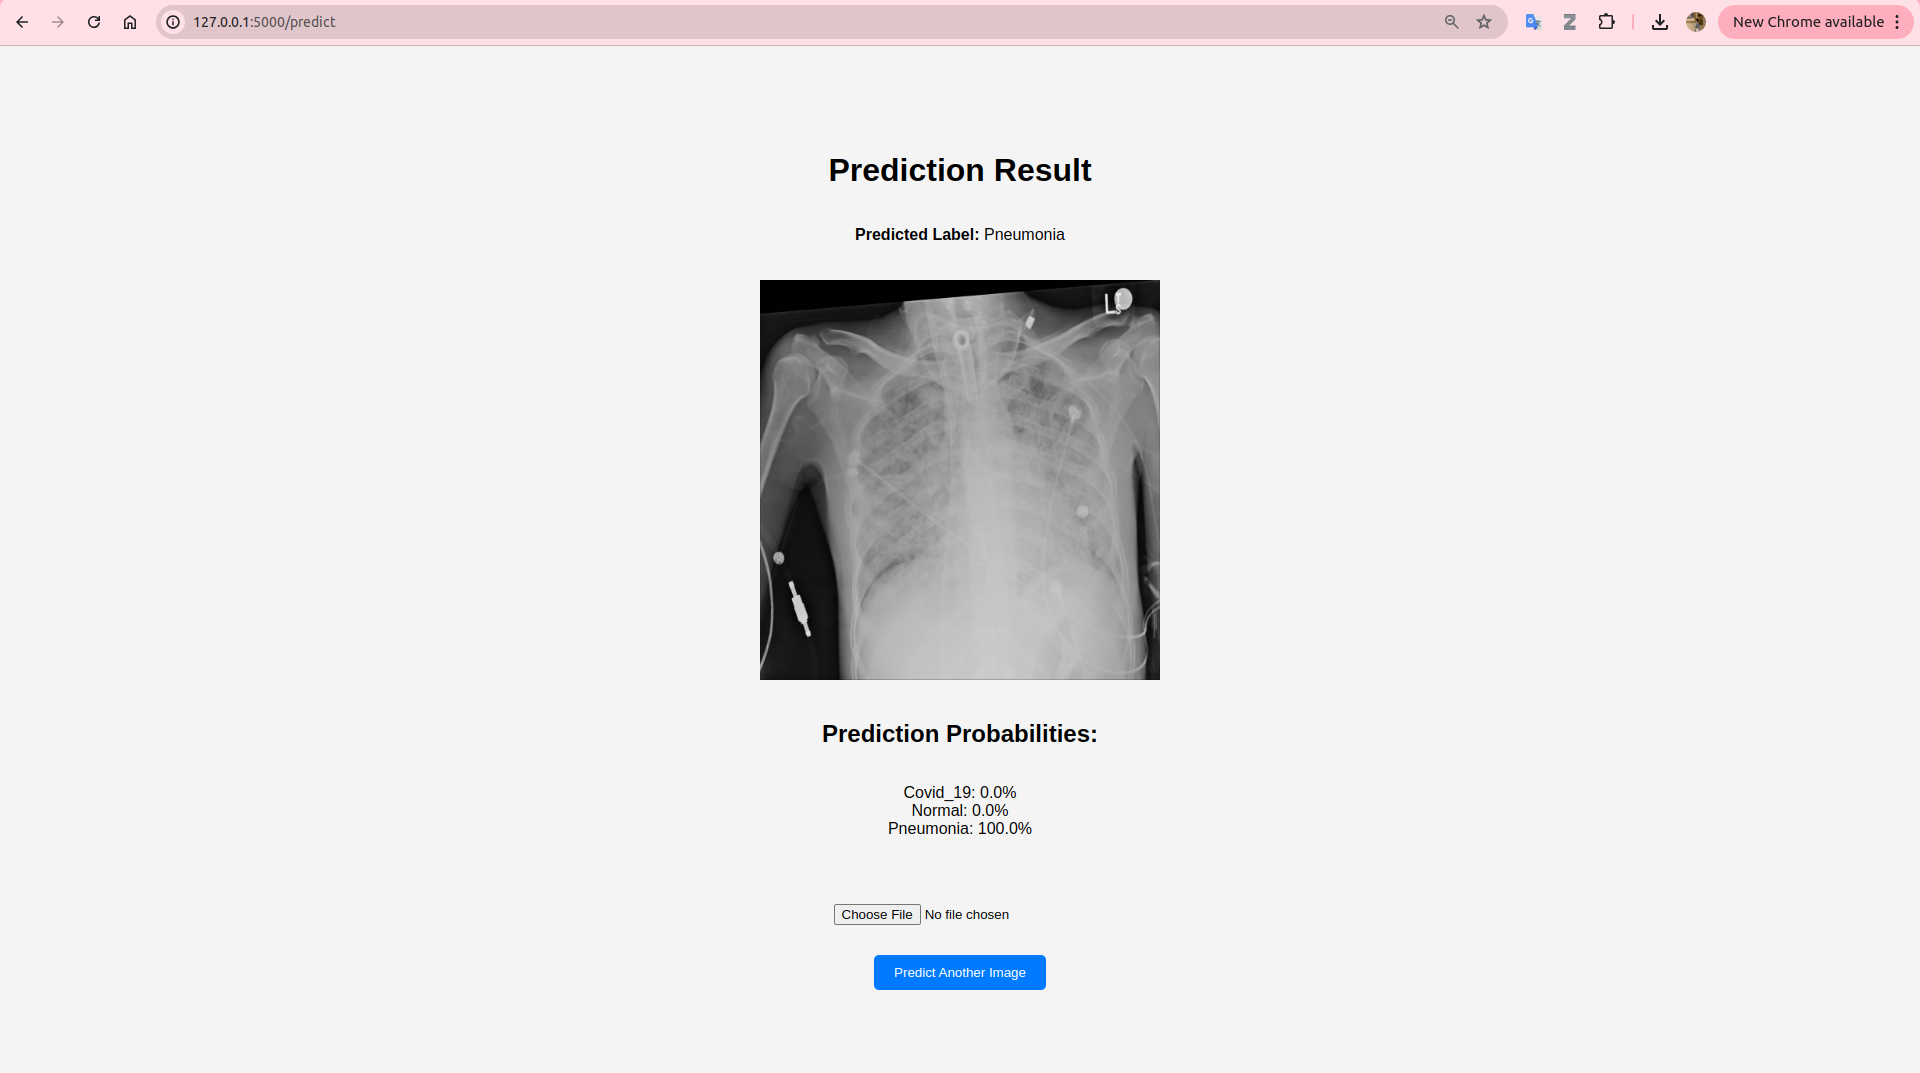
\includegraphics[width=\linewidth]{images/web2.png}
    \captionof{figure}{Result from the image using our source code.}
    \label{fig:output-code}
\end{minipage}
\end{center}

Demonstration on how to run our code can be found \href{https://drive.google.com/file/d/1xR-5_yizRXKgrdB_T-A1Rv4iwrHP8HVc/view?usp=drivesdk}{here}.

\section{Conclusion}
In this work, we have introduced an automated method for COVID-19 detection from chest X-ray pictures using deep learning. Our model successfully differentiates between Normal, COVID-19, and Pneumonia cases by using a mix of the Xception and ResNet50V2 networks as feature extractors. These findings show that deep learning methods, in particular convolutional neural networks, can significantly improve diagnostic precision, especially when prompt and accurate screening is required. The use of the Categorical Cross-Entropy loss function, as well as careful hyperparameter adjustment, have helped to improve the robustness and effectiveness of our model.

Though the outcomes are encouraging, there are a number of directions for further research. First, more comprehensive and diverse samples, particularly from underrepresented groups and various COVID-19 infection phases, can be included to the dataset. In order to further increase diagnostic accuracy, future studies may investigate the integration of other data modalities, such as CT scans or clinical information. Better decision-making comprehension for clinicians would be possible with the model's improved interpretability resulting from the application of explainable AI approaches. Lastly, a crucial first step in confirming the model's applicability and influence on public health would be to implement it in actual clinical settings.
\bigskip

\printbibliography

\end{document}